\documentclass{article}

\usepackage[a4paper]{geometry}
\usepackage{amssymb, amsmath, amsthm}
\usepackage{graphicx}
\usepackage{color}
\usepackage{lipsum}
\usepackage[T1]{fontenc}
\usepackage{subcaption}

\title{IM08: TP7}
\author{Felipe Vicentin}

\begin{document}
    \maketitle

    % Just submit a PDF with 1) an explanation of what \& how you did, 2) the Results.

    \section{Delaunay filtering conditions}
    The filtering conditions specify how to obtain an $\alpha$-shape from the Delaunay triangulation.
    To this end, we keep the triangles whose circumradius are smaller or equal than $\alpha$.
    For each triangle, we are given its endpoints in $\mathbb{R}^3$. And, to obtain the circumradius, we can use the following formula for the area of a triangle:
    \[
        A = \frac{a b c}{4 R}
    \]
    where $a, b, c \in \mathbb{R}$ are the lengths of the sides of the triangle and $R$ is the radius we are looking for.
    Thus,
    \[
        R = \frac{a b c}{4 A}.
    \]
    So, it suffices to compute $a, b, c$ and $A$.
    To do so, we can use the norm of the vectors defined by the endpoints of the triangle, i.e.,
    \begin{align*}
        a &= \| y - z \|_2 \\
        b &= \| x - z \|_2 \\
        c &= \| x - y \|_2,
    \end{align*}
    where $x, y, z \in \mathbb{R}^3$ are the endpoints of the triangle.
    After that, we can use a cross product in $\mathbb{R}^3$ to compute the area:
    \[
        A = \frac{\| (y - x) \times (z - x) \|_2}{2}.
    \]

    With that, we can finally compute $R$, and then filter out all triangles s.t. $R > \alpha$.
    The images below show some results for different alphas.

    \begin{figure}[htbp]
    \centering
    % First row of images
    \begin{subfigure}{0.3\textwidth}
        \centering
        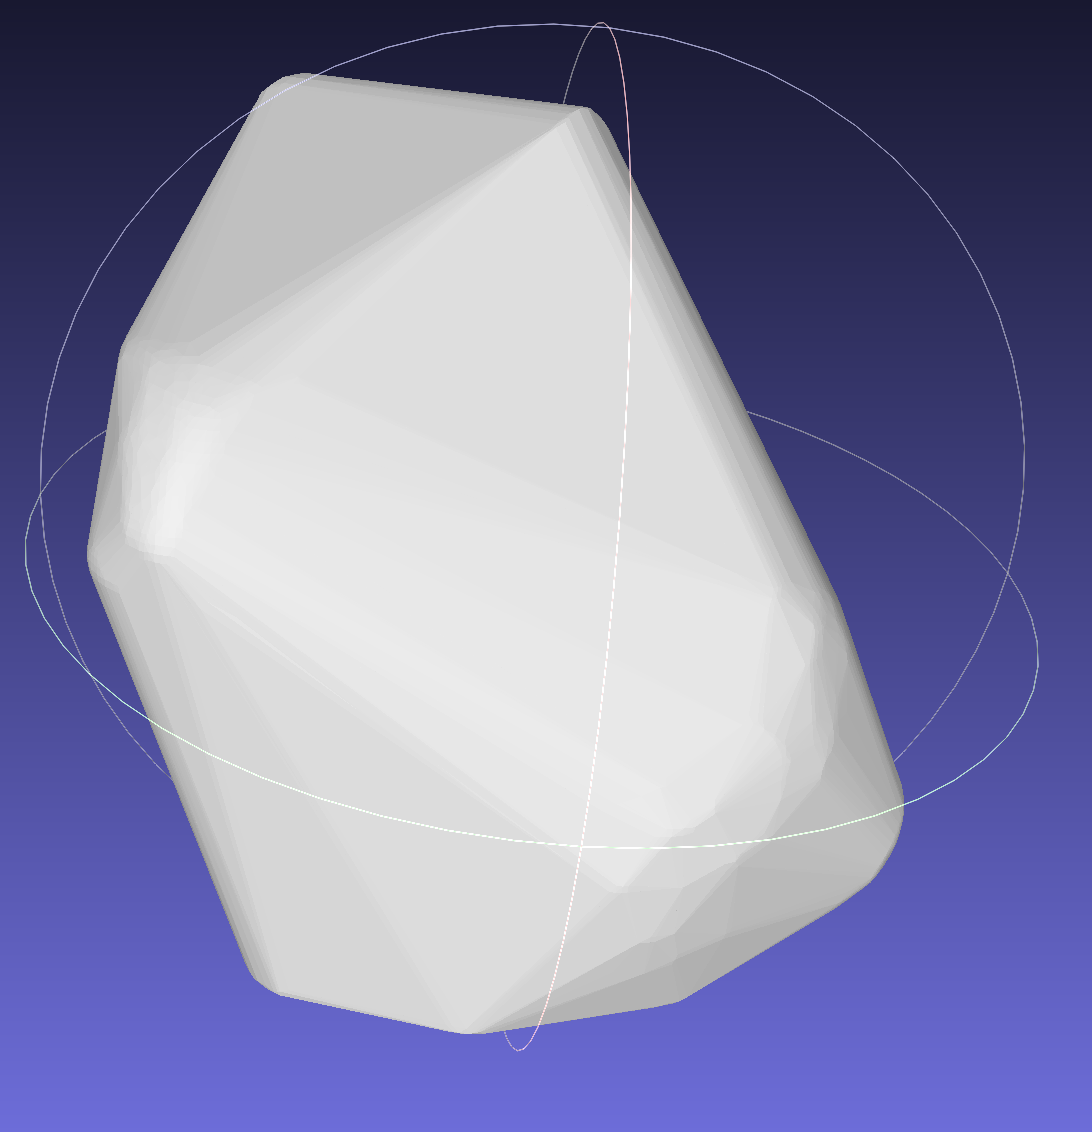
\includegraphics[width=\linewidth]{imgs/0_1}
        \caption{$\alpha = 0.1$.}
    \end{subfigure}
    \hfill
    \begin{subfigure}{0.3\textwidth}
        \centering
        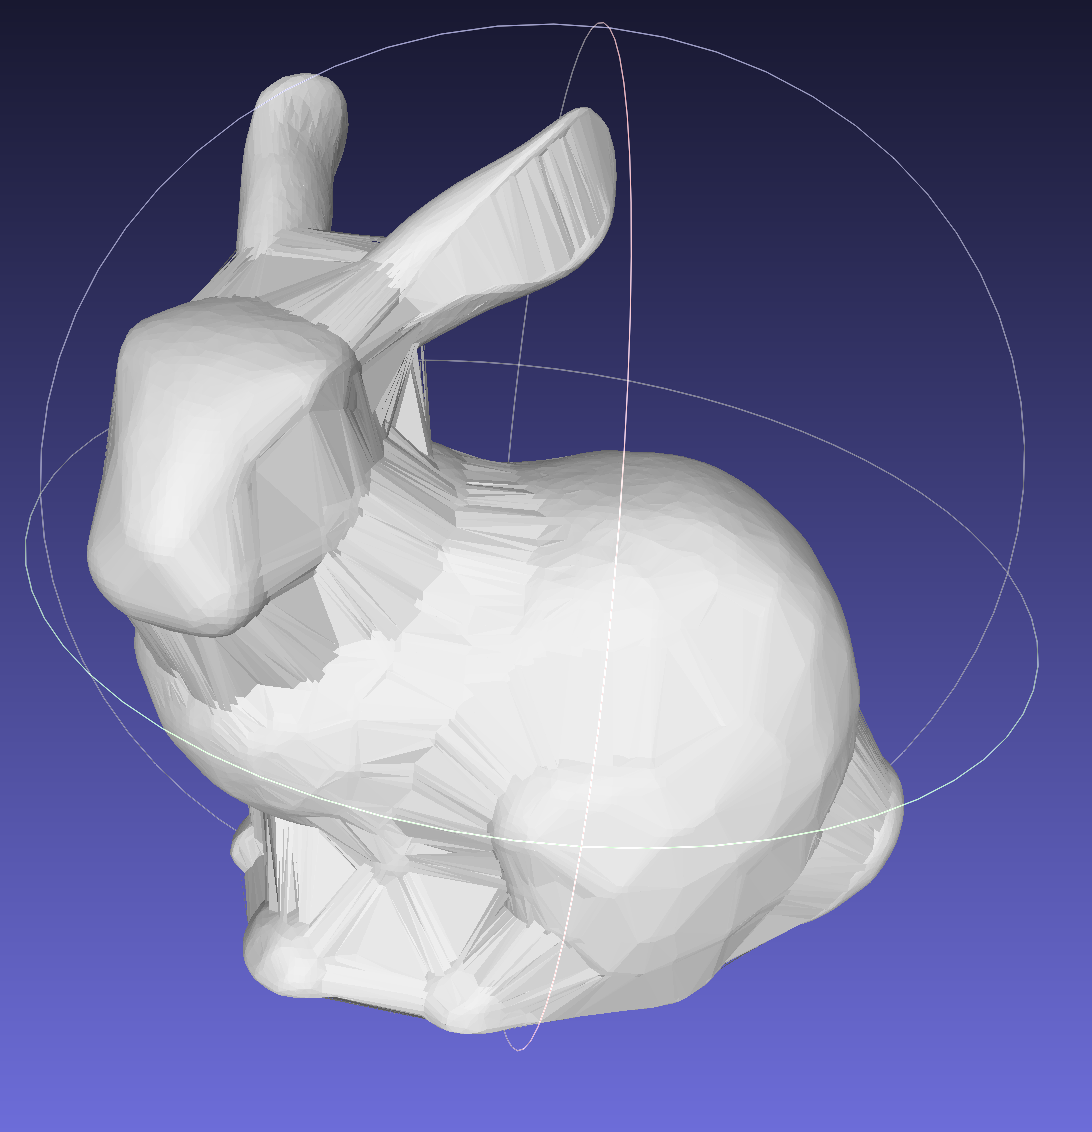
\includegraphics[width=\linewidth]{imgs/0_01}
        \caption{$\alpha = 0.01$.}
    \end{subfigure}
    \hfill
    \begin{subfigure}{0.3\textwidth}
        \centering
        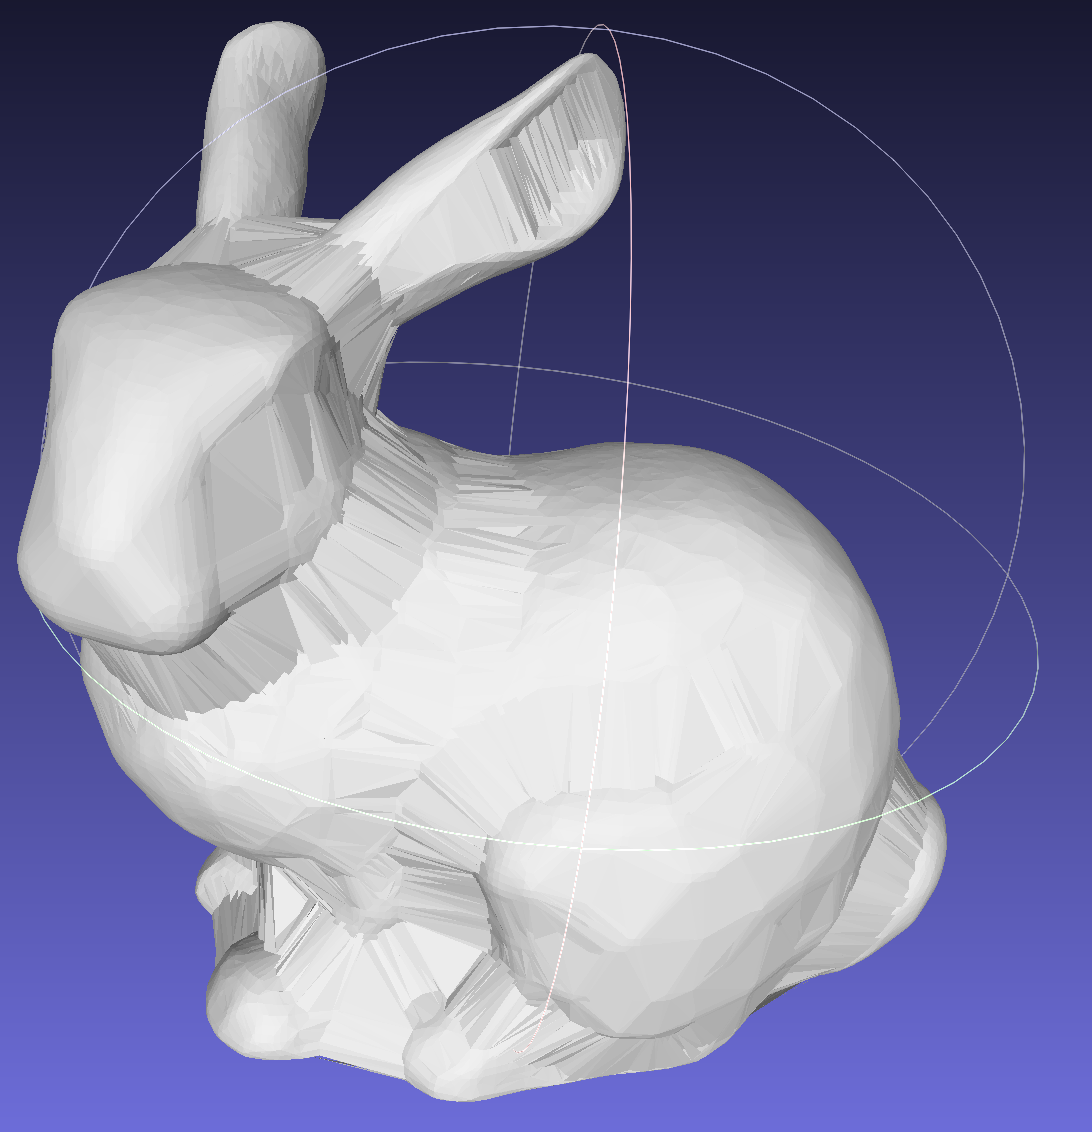
\includegraphics[width=\linewidth]{imgs/0_008}
        \caption{$\alpha = 0.008$.}
    \end{subfigure}

    \vspace{1em} % Adjust vertical spacing between rows

    % Second row of images
    \begin{subfigure}{0.3\textwidth}
        \centering
        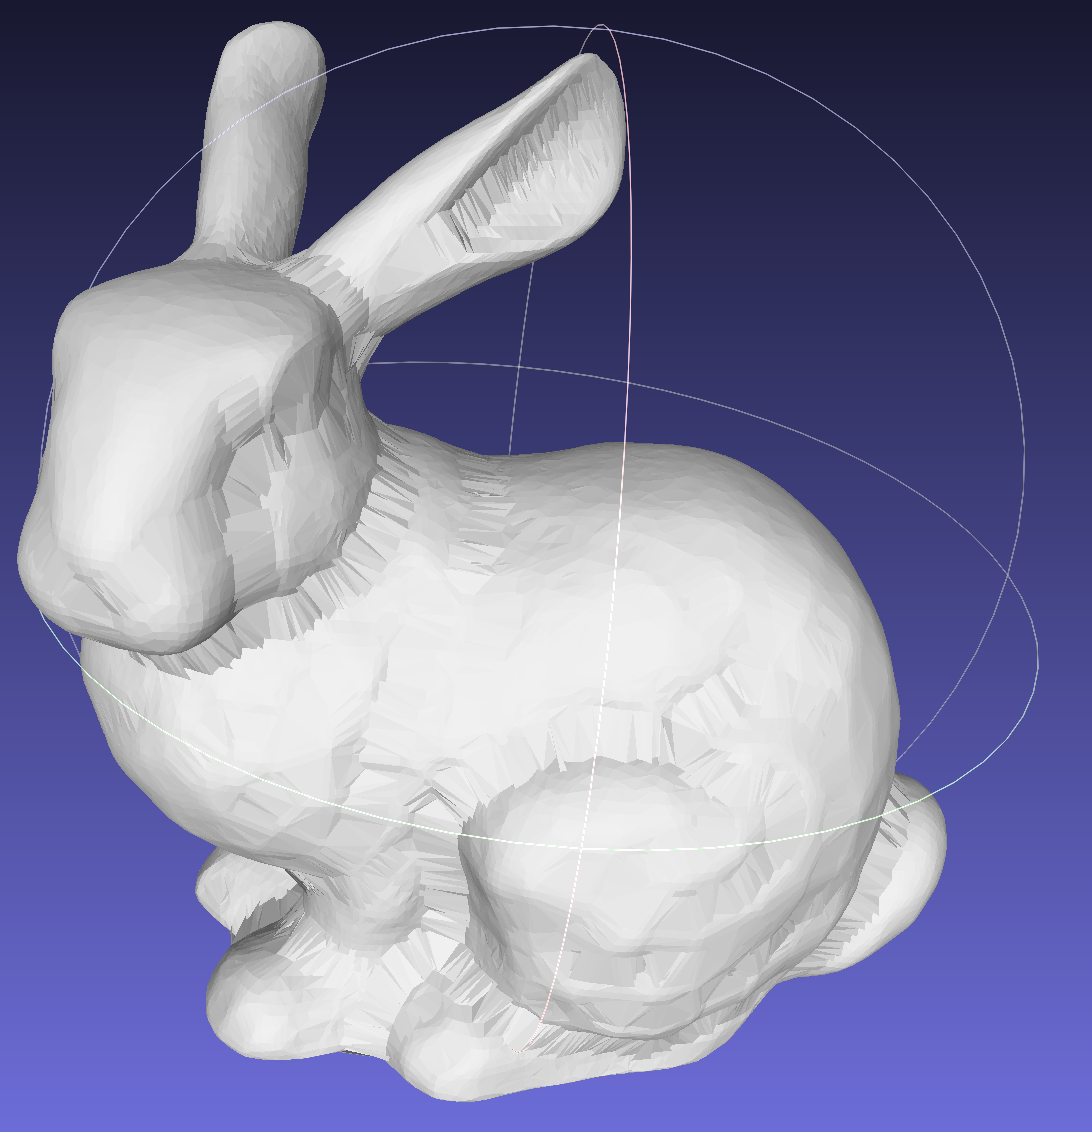
\includegraphics[width=\linewidth]{imgs/0_004}
        \caption{$\alpha = 0.004$.}
    \end{subfigure}
    \hfill
    \begin{subfigure}{0.3\textwidth}
        \centering
        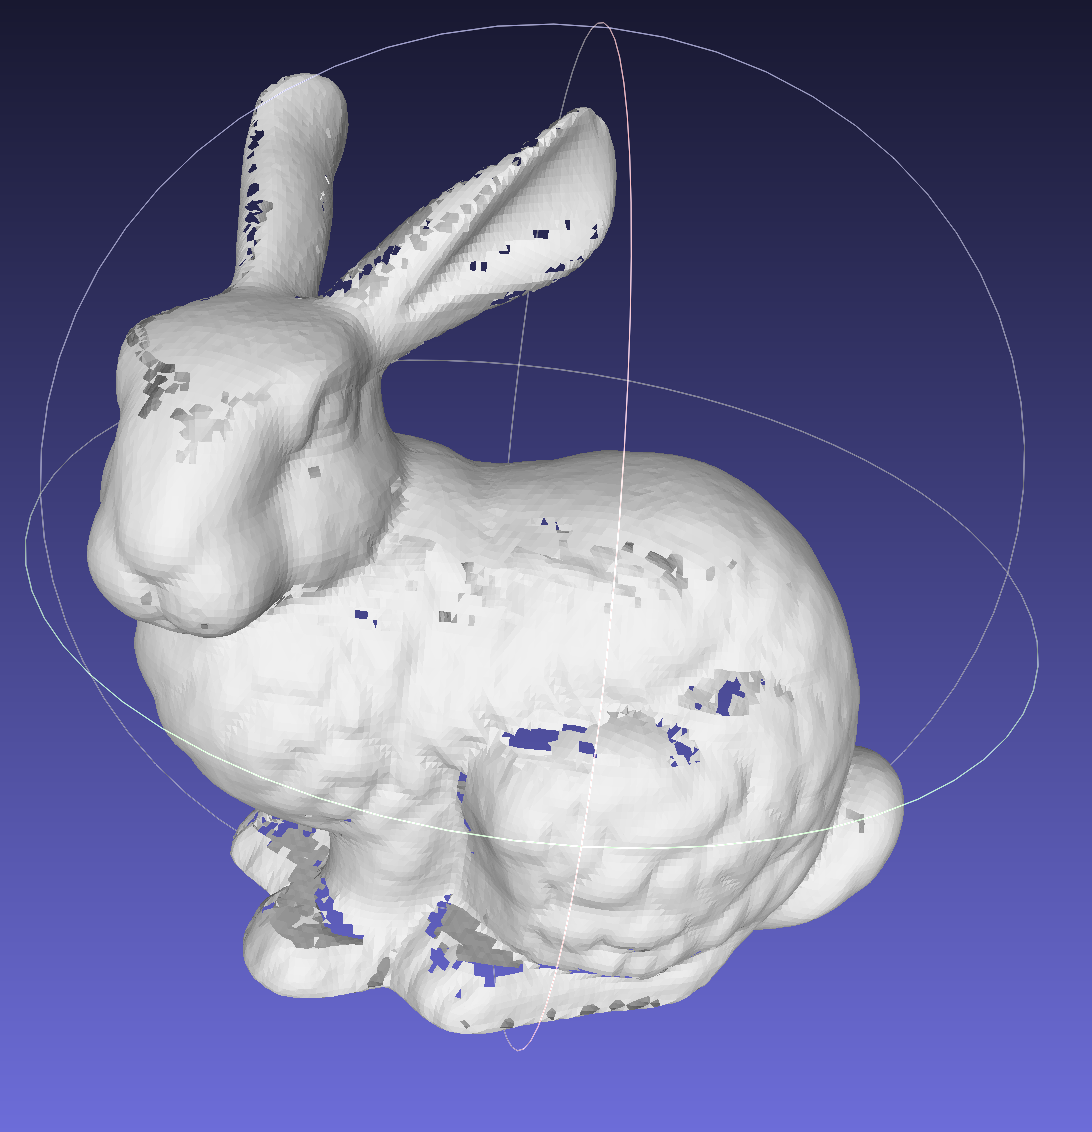
\includegraphics[width=\linewidth]{imgs/0_001}
        \caption{$\alpha = 0.001$.}
    \end{subfigure}
    \hfill
    \begin{subfigure}{0.3\textwidth}
        \centering
        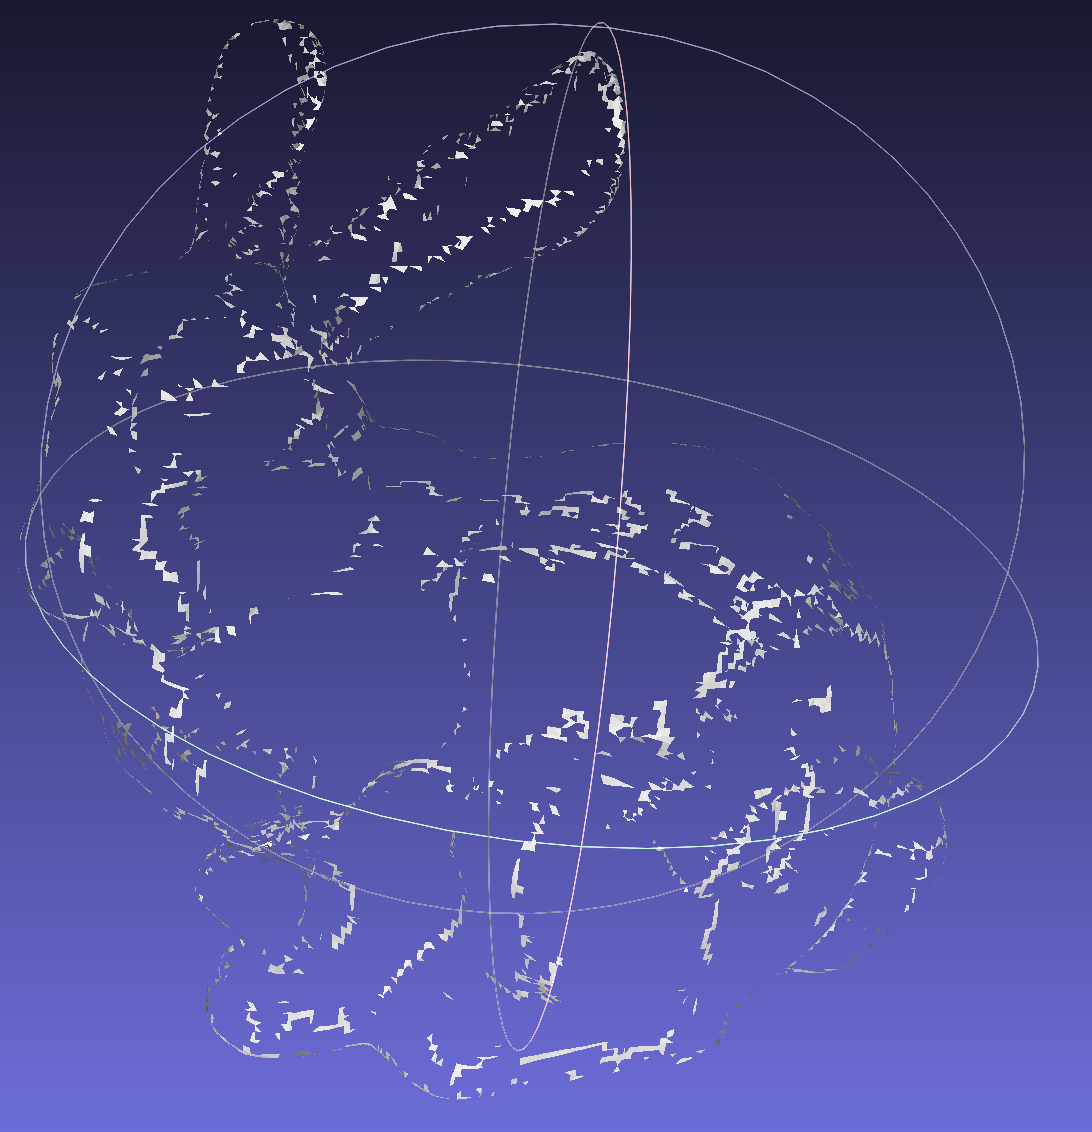
\includegraphics[width=\linewidth]{imgs/0_0008}
        \caption{$\alpha = 0.0008$.}
    \end{subfigure}

    \caption{Different $\alpha$ values for the filtering condition.}
\end{figure}

\end{document}

